\chapter{Aplikacje klienckie}

\section*{Aplikacja Android}

Opis Androida, screenshoty


\section*{Aplikacja iOS}

Opis iOS, screenshoty

Aplikacja przeznaczona jest na urządzenia z systemem operacyjnym iOS od wersji 10.0. 
Nie wspiera ona wcześniejszych wersji ze względu na nowe funkcje, które Apple wprowadziło wraz z pojawieniem się iOS 10.0 (m.in. klasa UNUserNotificationCenter). Jednak jak wynika z wykresu niżej (numer rysunku) 92\% wszystkich obecnych użytkowników tego systemu jest w stanie zainstalować aplikację a liczba ta stale rośnie. Aplikacja wykonana została wspierając zarówno telefony komórkowe iPhone jak i tablety iPad. 
\begin{figure}[h]
	\centering
	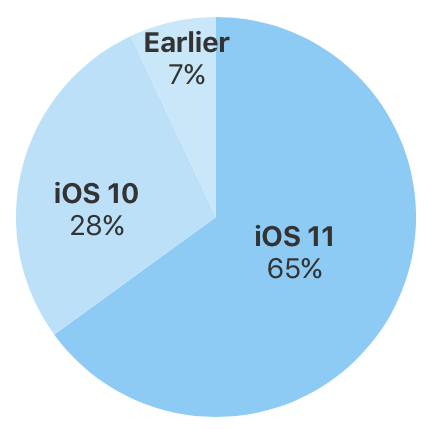
\includegraphics[width=6cm]{iOSstat}
	\caption{Udziały wersji systemu iOS w rynku}
\end{figure}

Architektura:
Aplikacja napisana jest w stosunkowo nowym języku Swift(został zaprezentowany przez Apple w 2014r na konferencji WWDC) w oparciu o architekturę MVC (Model-View-Controller) wykorzystując przy programowanie reaktywne i funkcjonalne. 
Programowanie reaktywne wykonane zostało przy pomocy biblioteki RxSwift. Wykorzystano je m.in w celu wznowienia streamu obrazu z kamery w momencie przejścia aplikacji z trybu Background do trybu Foreground. Oznacza to, że w momencie wyjścia z aplikacji ale pozostawiając ja działającą w tle i po chwili uruchomienia jej ponownie traciliśmy obraz Video, ze względu na politykę bezpieczeństwa Apple, która nie zezwala aby aplikacje pobierały dane przez dłuższy okres czasu kiedy aplikacja pracuje w tle. Dzięki programowaniu reaktywnemu problem ten został rozwiązany co prezentuje poniższy kod:
\begin{verbatim}
let appDelegate = UIApplication.shared.delegate as! AppDelegate
        appDelegate.inBackground.asObservable().subscribe(onNext: { (value) in
            if let streamView = self.streamView {
                if let player = self.currentPlayer {
                    if value == false {
                        self.streamVideoFrom(urlString: self.currentUrlString!)
                        print("Enter foreground")
                    } else {
                        print("Enter background")
                        streamView.layer.sublayers?.forEach({ (layer) in
                            layer.removeFromSuperlayer()
                        })
                    }
                }
            }
        }).disposed(by: disposeBag)
\end{verbatim}
Zmienna inBackground ustawiana jest oddzielnej klasie AppDelegate na wartość true kiedy aplikacja przechodzi w tryb background i na wartość false w przeciwnym wypadku. Kod powyżej uruchamia się za każdym razem przy zmianie tej wartości i uruchamia stream po każdym ponownym uruchomieniu programu.
Instalacja zewnętrzynych bibliotek odbywa się za pomocą CocoaPods. Jest to menadżer zależności dzięki któremu szybko możemy wyszukać i zainstalować wymagane oprogramowanie.

Po uruchomieniu aplikacji pierwszym widokiem jest ekran logowania i rejestracji użytkowników(rys 5.2).
\begin{figure}[h]
	\centering
	
\includegraphics[width=6cm]{login.png}
	\caption{Ekran logowania}
\end{figure}

Po prawidłowej autoryzacji danych użytkownika wprowadzonych podczas logowania ukaże się nam główny widok aplikacji. W górnej części mamy do wyboru 5 sekcji:
sekcja czujników, sekcja historii notyfikacji, sekcja zagrożeń przy wykryciu ruchu, sekcja streamu na żywo, sekcja ustawień. Wszystkie te sekcje dotyczą konkretnego urządzenia wybranego w opcjach na dole ekranu. Początkowo przy pierwszym uruchomieniu nie będziemy posiadali żadnych urządzeń przypisanych do naszego konta użytkownika. Aby dodać pierwsze i kolejne stacje, od których chcemy otrzymywać notyfikacje o zagrożeniach a także śledzić i monitorować informacje z czujników należy wybrać przycisk "New" z plusikiem w dolnej części ekranu. Pojawi się okno z prośbą o wpisanie numeru identyfikującego jednoznacznie urządzenie. Po chwili dodany Guard będzie widoczny w na liście.

\paragraph{Sekcja czujników:}
Jest to jedna z najważniejszych sekcji aplikacji (rys 5.3).  Otrzymuje ona dane z czujników w czasie rzeczywistym i prezentuje je użytkownikowi.  W zależności od koloru prezentowanej wartości z czujnika użytkownik analizuje zagrożenie. Kolor zielony reprezentuje bezpieczne i prawidłowe odczyty na czujnikach, kolor pomarańczowy średnie, kolor czerwony reprezentuje bardzo wysoki poziom niebezpieczeństwa. Implementacja tej funkcjonalności zrealizowana została przy pomocy modelu HSV a nie RGB, dzięki temu zmieniając parametr Hue zmieniamy barwę przy stałym nasyceniu i jasności. Wartość tego parametru równa 120\textdegree{} odpowiada kolorowi zielonemu, kolor czerwony to 0\textdegree{}. Przekształcając wartość otrzymaną z czujników, która jest z zakresu [0-1] na wartość z przedziału [120-0] otrzymano wyżej wspomniany efekt. 
Poniżej przedstawiono fragment konwersji danych z czujników na kolor w modelu HSV, gdzie zmienna sensors[0] reprezentuje czujnik LPG.
\begin{verbatim}
UIColor(hue: CGFloat(0.33 - (sensors[0].value * 0.33)),
saturation: 1, brightness: 1, alpha: 1)
\end{verbatim}

\begin{figure}[h]
	\centering
	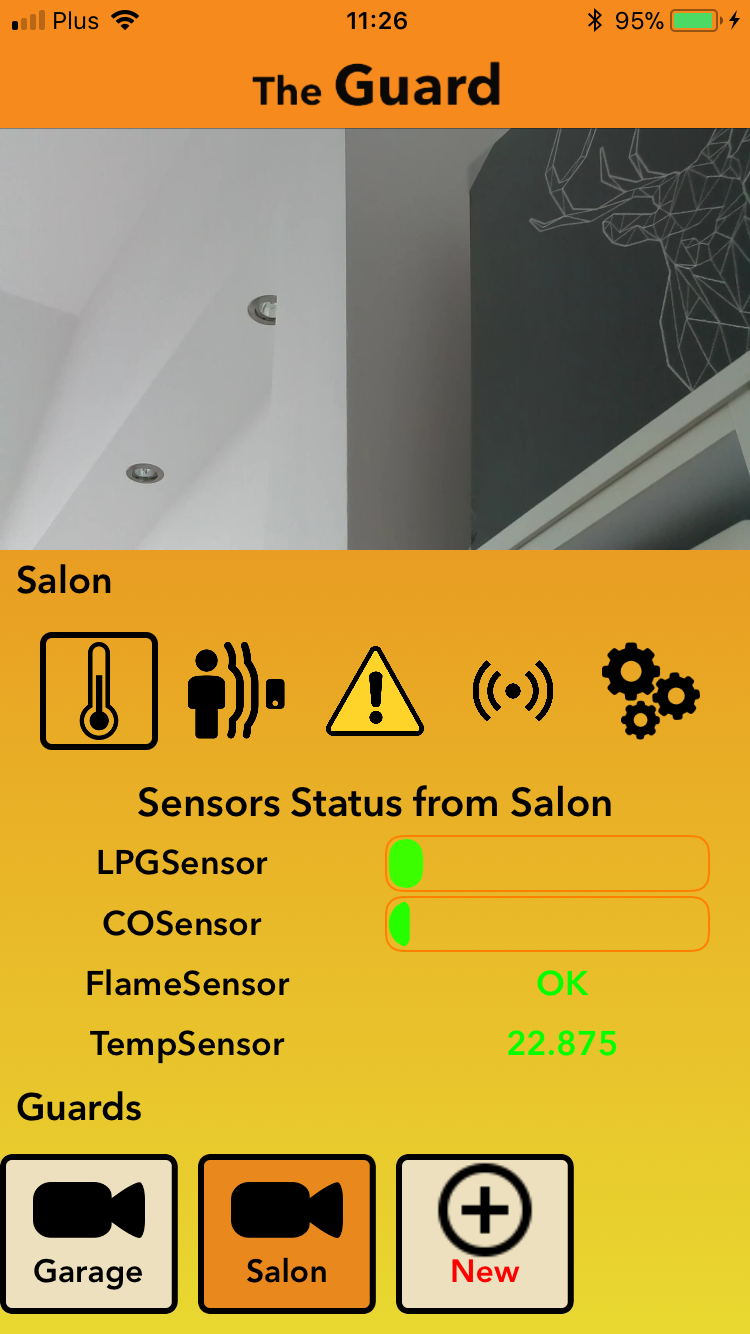
\includegraphics[width=6cm]{sensors.png}
	\caption{Sekcja czujników}
\end{figure}

\paragraph{Sekcja historii notyfikacji:}
W tej sekcji użytkownik ma dostęp do historii zdarzeń w systemie (rys 5.4). Po zaznaczeniu interesującego nas daty reprezentującej moment wystąpienia zagrożenia prezentowna jest informacja o miejscu niebezpieczeństwa i jego rodzaju.

\begin{figure}[h]
	\centering
	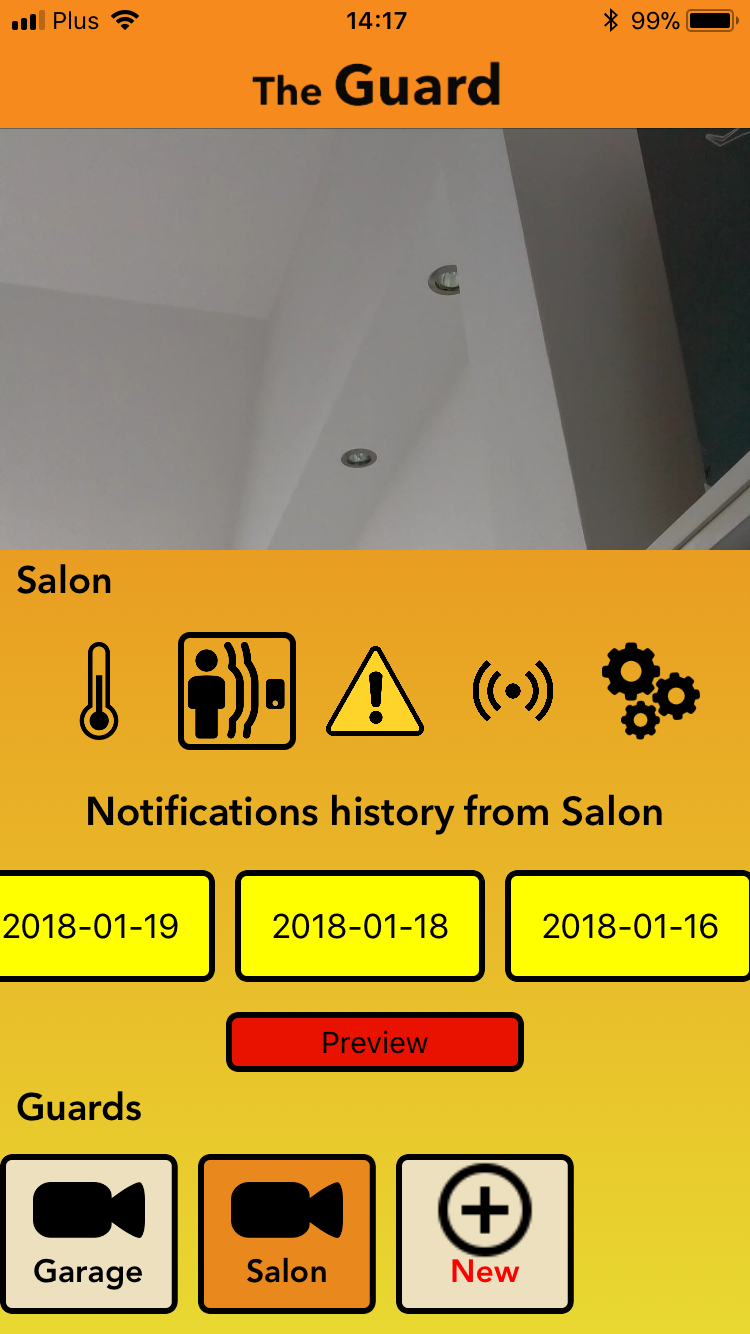
\includegraphics[width=6cm]{history.png}
	\caption{Sekcja historii zdarzeń}
\end{figure}


\paragraph{Sekcja ustawień:}
Ustawienia dotyczące zaznaczonego na dole ekranu urządzenia (rys 5.5). Użytkownik ma możliwość zmiany nazwy urządzenia, które zazwyczaj reprezentuje miejsce, w którym znajduje się stacja pomiarowa. Istnieje również możliwość uzbrojenia i wyłączenia konkretnego czujnika. Sprowadza się to do tego, że w przypadku zaznaczenia opcji "Disarmed" użytkownik nie będzie otrzymywał kolejnych notyfikacji o zagrożeniach. Opcja ta może okazać się przydatna w momencie uszkodzenia któregoś z modułów i tym samym błednych danych wysyłanych z czujników.

\begin{figure}[h]
	\centering
	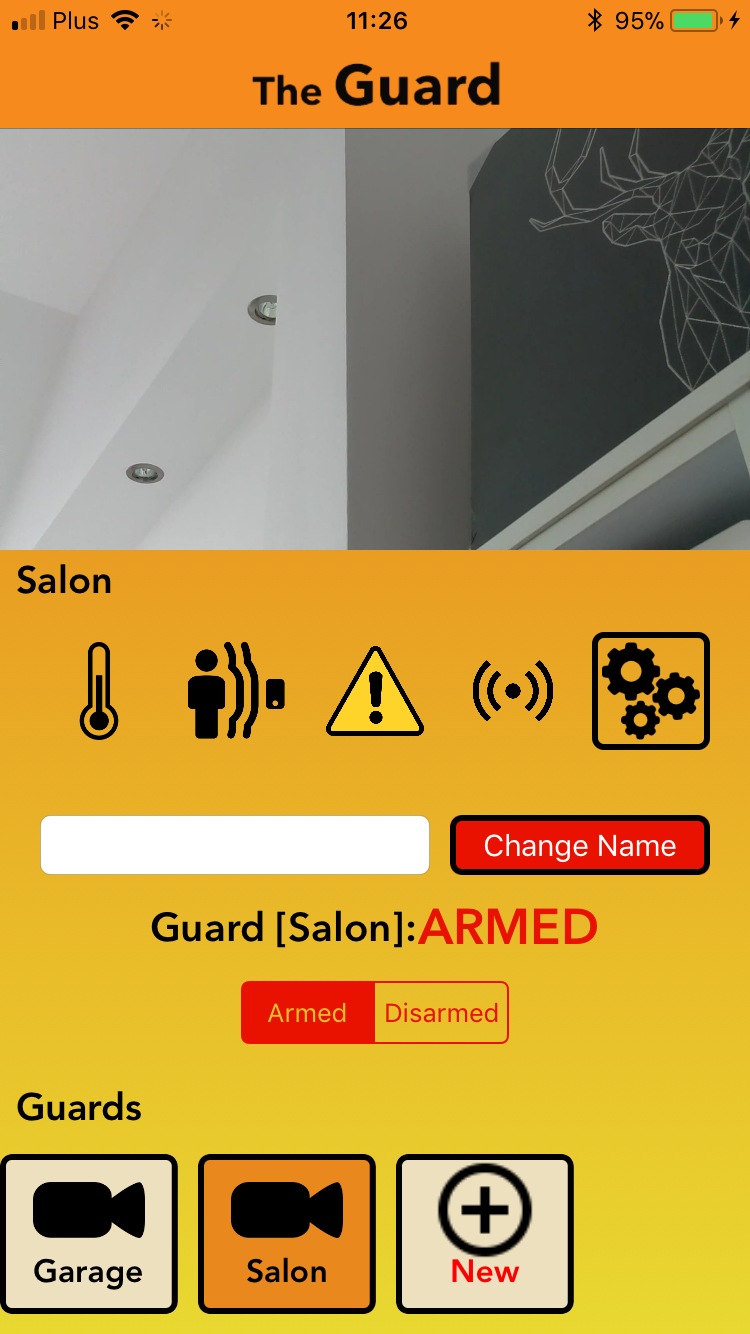
\includegraphics[width=6cm]{settings.png}
	\caption{Sekcja historii zdarzeń}
\end{figure}








\section*{Aplikacja internetowa}

Opis weba, screenshoty